\documentclass[10pt,twoside,twocolumn,openany]{book}

% The following packages were required to make the dnd.sty work
\usepackage[table]{xcolor}
\usepackage{tikz}
\usepackage{everyshi}
\usepackage{keycommand}
\usepackage{fancyhdr}
\usepackage[most]{tcolorbox}
\usepackage{environ}
\usepackage{trimspaces}
\usepackage{fp}
\usepackage[pages=all]{background}
\usepackage{everypage}
\usepackage{listings}

\usepackage[bg-letter]{dnd} % Options: bg-a4, bg-letter, bg-full, bg-print, bg-none.
\usepackage[english]{babel}
\usepackage[T1]{fontenc}
\usepackage{lmodern}
\usepackage[utf8]{inputenc}
\usepackage{graphicx}

\usepackage{datetime}
\usepackage{amssymb}

\usepackage{hyperref} % these two lines are so that the table of content is clickable
\hypersetup{linktoc=all}
%\setlength{\parindent}{0pt}

\begin{document}
	\begin{titlepage} % good tital page template, only needs the class X notes part to be changed for each new class
		
		\centering
		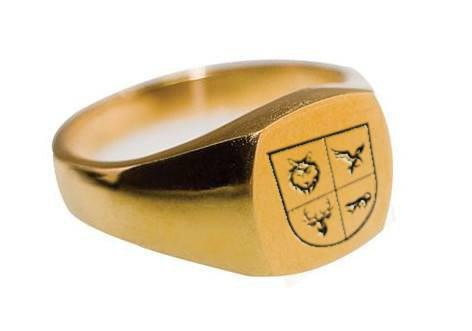
\includegraphics[width=0.40\textwidth]{NandirLogo}\par\vspace{1cm}
		{\scshape\LARGE Nandir Abenteuer \par}
		\vspace{1cm}
		{\huge\bfseries Die Theatergruppe \par}
		\vspace{2cm}
		{\Large\itshape by Lysanthir \par}
		
		\vfill
		
		% Bottom of the page
		
	\end{titlepage}
	
	\tableofcontents % creats a table of contents, ensured already that it is clickable
	\newpage % starts the actual document on a new page so there is no weird colision of text and toc
	
	\chapter{Backstories}
	
	\section{Sarasaus}
	
	\newpage
	\section{Taria}
	
	\newpage
	\section{Dalothor}
	
	\newpage
	\section{Prun}
	Prun ist ein junger Elf, welcher sich an seinem derzeitigen Herrscher rächen will. Er war in seiner Kindheit ein guter Freund des Thronfolgers und lebte mit seiner Familie am Hofe des Fürsten. Doch nach dessen Sturz wurde er von dem neuen, bösen Hofmagier entführt. Dieser führte grausige magische Experimente an ihm und anderen „Testsubjekten“ durch, um seine Wissenschaft voranzutreiben. Eines Tages ging eines seiner Experimente schief, und eine riesige Explosion riss die Burg des Magiers und viele der dortigen Wesen in Stücke. Prun überlebte die Explosion und machte seinen Weg an vielen verkohlten Leichen vorbei in seine neugewonnene Freiheit. Nun will er Rache nehmen an dem neuen Fürsten und dem Magier, sollte er überlebt haben. Sein erstes Ziel ist es, seinen alten Freund und rechtmäßigen Thronfolger zu finden und ihm zu seinem rechtmäßigen Platz zu verhelfen.
	
	\newpage
	\section{Lysanthir}
	
	Lysanthir ist mit seinen Eltern im Wald von Langorion mit Elfen groß geworden. Seine gesamte Kindheit verbrachte er damit, mit den anderen Elfenkindern zu trainieren. Eines Tages beim Jagen fing eine Eule an, ihm Beute zu finden, welche er erlegen konnte. Die erlegte Beute teilte er mit der Eule. Nach einigen Wochen dieser Vorgehensweise freundeten sie sich an. Die Eule wurde Oreo getauft. Seitdem arbeiteten sie als koordiniertes Team, um Beute zu Sammeln. Trotz der engen Verbindung der beiden haben sie jeweils kein Problem damit Tage lang ihr eigenes Ding durchzuziehen. 
	
	Vor zwei Jahren, als der alte Fürst gestürzt wurde, hat der neue Fürst beschlossen seine Macht zu demonstrieren, indem er in den Wald ging und einige der Bewohner des Waldes töten ließ. Unter den unglücklichen waren Lysanthirs Eltern. Seit diesem Tag trainiert Lysanthir nicht nur um ein besserer Jäger zu werden, sondern nun auch um den neuen Fürsten zu erlegen. Unter den Waldbewohnern ist Lysanthir als grüner Umhang bekannt, da man ihn nur noch in seinem Mantel sieht. 
	
	[TODO: continue appearance description]

	Eines Tages beim Jagen bemerkt Lysanthir eine Explosion am Rande des Waldes. Frustriert, da die Beute durch das laute Geräusch Angst gefüllt entkommen ist, untersuchte Lysanthir den Ursprung der Explosion. Auf dem Weg rennt ihm Prun über den Weg, welcher Lysanthir rekrutierte, um zu versuchen den Fürsten zu stürzen.
	
	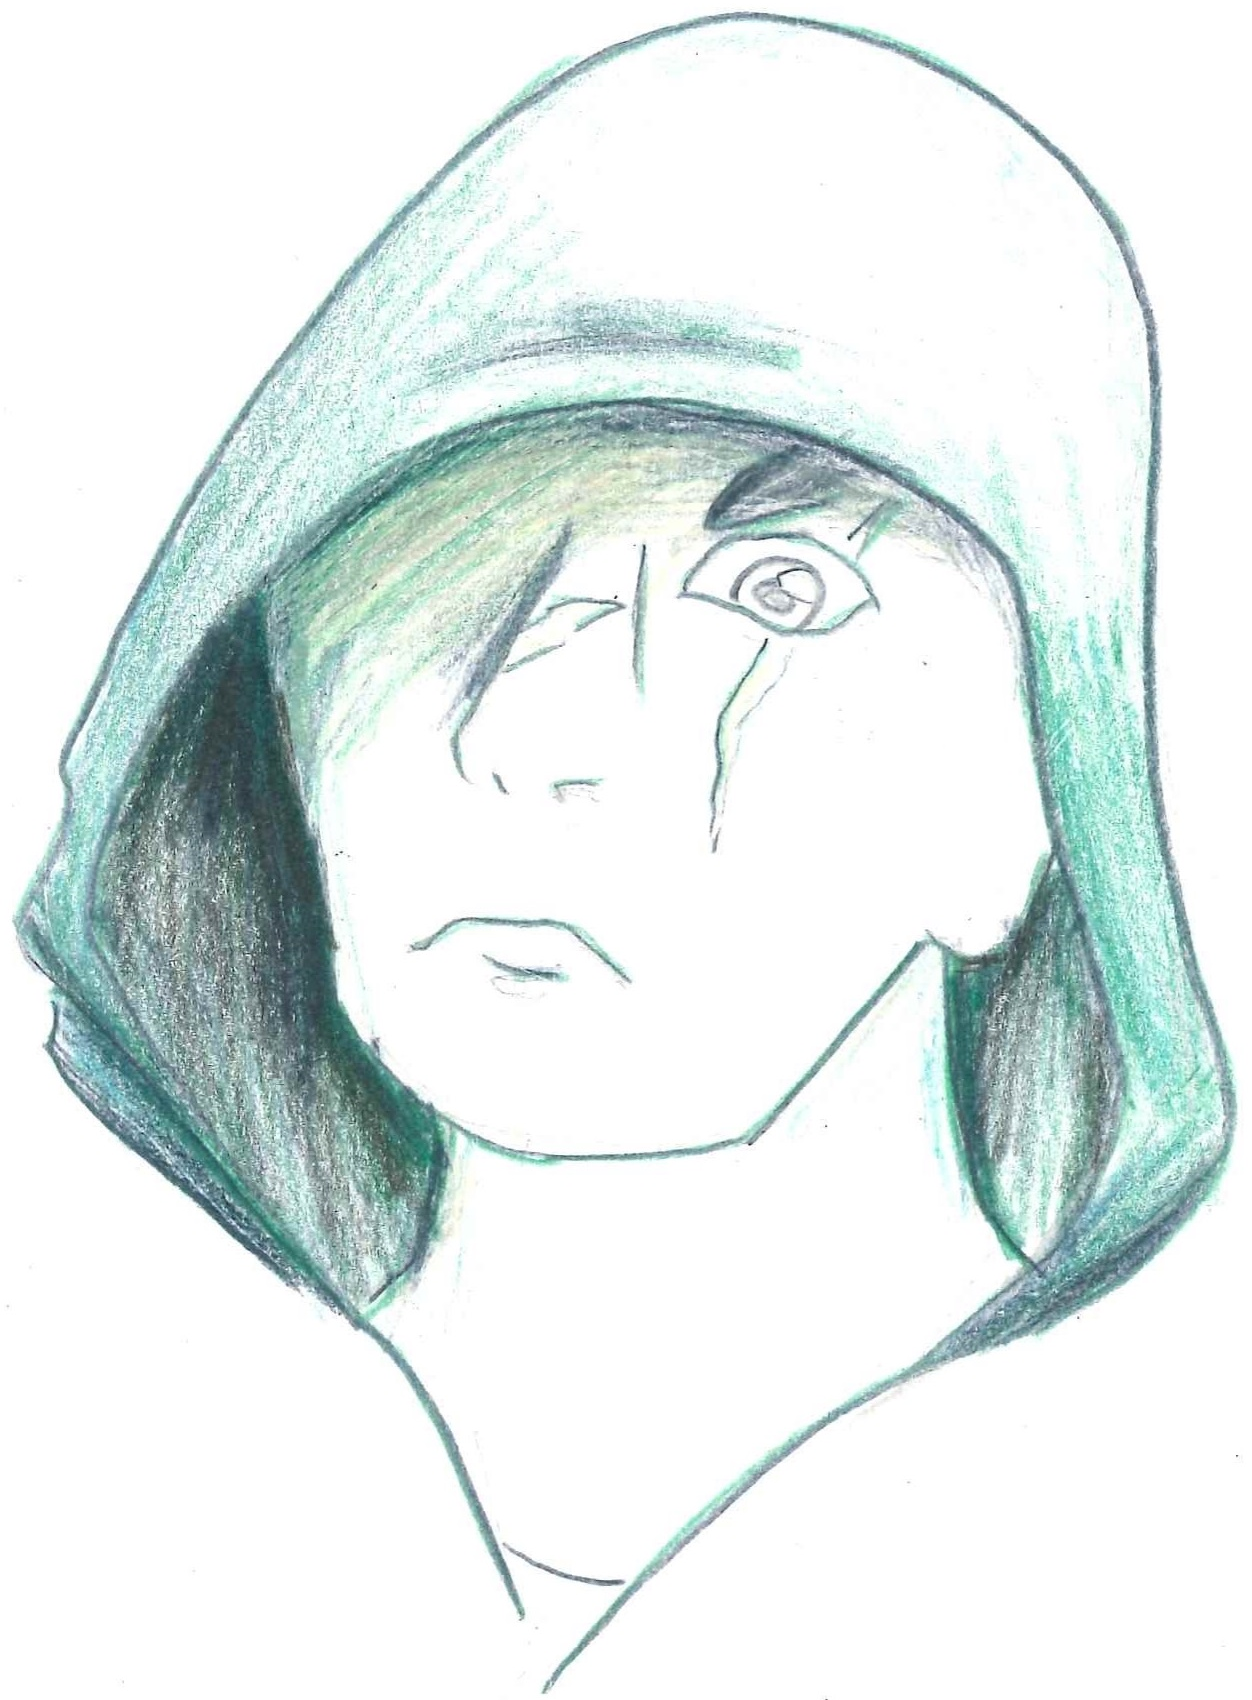
\includegraphics[width=0.40\textwidth]{LysanthirFace}\par
	\includegraphics[width=0.40\textwidth]{Lysanthir}\par\vspace{1cm}
	\newpage
	
	\chapter{Session eins}
	
	\section{Der Informant}
	
	Gruppe trifft einen Informanten der gegen einen Ring Information tauschen will.
	Prun weiß von diesem Ring da er seiner Familie gehörte.
	2 Tage bis der Ring übergeben werden soll.
	Die Gruppe trennt sich in zwei Gruppen auf, Taria und Dalothor sollen auf der Straße die Wachen ablenken. In der Zwischenzeit werden Prun und Sarasaus in das Haus einbrechen, was nun nicht mehr von Wachen umzingelt sein wird, während Lysanthir draußen den Weg frei halten soll.
	
	\section{Die Ablenkung}
	
	Taria und Dalothor klettern unauffällig aus der Kanalisation und schauen sich um. Sie merken, dass hinter ihnen eine Schmiede ist. Für den Aufstand wollten sie eine Fackel, gehen also in die Schmiede und fragen nach einer Fackel. Der Eigentümer möchte ihnen erstmals nicht helfen und bittet sie zu gehen. Dalothor befiehlt dem Besitzer ihm eine Fackel zu geben. Nach kurzem Einwirken des Befehls reicht der Lehrling Dalothor eine Fackel. Mit Fackel in der Hand machen die beiden sich auf den Weg zu einem mehr zentral gelegenen Ort um für Aufruhr zu sorgen. 

	Taria fängt an laut auf der Straße zu predigen und die Aufmerksamkeit der Menschen auf sich zu ziehen. Trotz zuvor gut gelaufenen Predigen, läuft diese nicht wie geplant. Die Menschenmassen - welche sich um die zwei bilden - sind mehr empört von dem was Taria zu sagen hat, als entzückt, fangen deshalb an mit Obst nach ihr zu werfen. In der Zwischenzeit machen sich mehr und mehr Speere durch die Masse Richtung Taria und Dalothor, die Wachen kommen nun um die Ursache der Menschenmasse zu beseitigen. Vorne angekommen werden Taria und Dalothor befragt was sie machen und befehlen ihnen deren Waffen abzugeben, da Waffen in der Stadt verboten sind. Kurz bevor ein Kampf in der Straße ausbricht, landet ein Dachziegel vor Tarias Füßen. Instinktiv schauen alle, die den Dachziegel bemerkt haben auf das Dach, von dem er geworfen wurde und sehen eine in einem grünen Mantel eingehüllte Person. welche ein Signal zu geben scheint und dann über die Dächer verschwindet. Taria und Dalothor haben erkannt, dass sie nicht mehr für Unruhe sorgen müssen und versuchen wieder zum Gullydeckel zu gelangen. Auf dem Weg bewegen sich einige Wachen zwischen ihnen und dem Gullydeckel, sind jedoch nicht ganz schnell genug, wodurch die beiden in die Kanalisation abtauchen können. Unten angekommen machen sie sich kampfbereit, um jede Wache, welche von oben runter zu kommen versuchen wolle, abzufangen. 

	Nach einiger Zeit, in der die Wachen erfolglos mit Speeren nach Dalothor stachen, hörte Taria hinter ihr, dass es einige in die Kanalisation geschafft hatten. Sofort drehte sie sich um und sah wie drei Wachen sich ihnen näherten. In einem Versuch, sie zu stoppen, stürmte sie in Richtung der Wachen und zog ihr Schwert. Leider war der Untergrund etwas zu schmal und ihr Schwert blieb in der Wand stecken. Dalothor stürmt auf eine der Wachen und tötet sie mit einem kräftigen Hieb. Bei der zweiten Wache hatte er nicht so viel Erfolg und rutschte aus. In einem Versuch ihr Schwert raus zu ziehen, sorgt sie dafür, dass der Tunnel anfängt zusammen zu stürzen. Ohne Grund mehr in dem Tunnel zu stehen fangen sie an vor den Wachen und dem einstürzenden Tunnel zu fliehen. 

	Sie entscheiden sich, dass sie zurück zur Taverne müssen und auf die anderen warten werden, fangen also an, sich in Richtung des Faulen Apfels sich zu begeben. Sie bemerken, dass die Wachen ihnen schon auf den Fersen sind. Auf dem Weg sehen sie eine Abzweigung, welcher sie folgen, um die Wachen abzuschütteln. Leise machen sie sich bis zum Ende des Ganges, wo sie auf eine Wand treffen. Dalothor bemerkt, dass die Wand vor ihnen nicht so alt ist wie die anderen. Da erinnerte sich Taria an etwas, das jemand aus der Taverne zuvor gesagt hatte, dass auf einmal eine Wand einen Weg, der zur Taverne führt, blockiert. Sie vermuten, dass es sich hier um diese Wand handelt und brechen Schild zuerst durch die Wand. Auf der anderen Seite der Wand scheint eine Art Tresor zu sein. Um das Licht in dem Tresor von der anderen Seite zu verstecken verschieben sie ein Bücherregal vor das Loch und hoffen so, unauffällig bleiben zu können. Mit dem Bücherregal vor dem Loch hatten sie endlich Zeit sich umzusehen. Taria bemerkte eine Schatulle auf dem verschobenen Regal und steckte diese ein. Nach einer kurzen Pause bemerken sie ein Geräusch von der anderen Seite der Tresor-Tür. Flüchtig versucht Dalothor das Bücherregal um zu rennen, um wieder auf die andere Seite der Wand zu gelangen. Dies scheiterte nur, da er ausrutschte. Sein Fall sorgte dafür, dass er sich ausknockte. Da das Tresor seid Einbruch der Stimmen immer noch nicht geöffnet wurde, versucht Taria den Tresor von der anderen Seite zu öffnen. Leider kannte sie sich nicht gut mit Tresoren aus, und löste eine interne Falle aus, welche dafür sorgte, dass die Decke langsam auf sie und Dalothor sich senkte. 
	
	\section{Thaeder Familienanwesen}
	
	Eine Station weiter warten Prun, Sarasaus, und Lysanthir darauf, dass die Wachen sich vom Haus entfernen, um das Haus zu infiltrieren. Sie hören, wie Taria und Dalothor die Rede beginnen und wie die Wachen sich vom Haus entfernen. Lysanthir wird voraus geschickt, um zu schauen, ob die Luft rein ist. Er klettert hoch und sieht nur ein kleines Mädchen. Die Mutter und sie schauen ihn verstört an und gehen weiter. Lysanthir signalisiert den anderen beiden dass sie hinauf kommen können. Prun und Sarasaus machen sich auf zum Anwesen, während Lysanthir sich auf das nächstgelegene Dach begibt. 
	
	\subsection{Lysanthirs Entkommen}
	
	Nach einiger Zeit kommt Sarasaus kurz aus dem Haus und signalisiert Lysanthir, dass er die anderen beiden informieren soll, dass sie sich weg begeben können, wenn sie wollen. Nachdem Sarasaus wieder ins Haus geht, macht sich Lysanthir auf zu einem Punkt, von welchem aus er Taria und Dalothor gut sehen kann. Nach kurzer Überlegung - vielleicht zu kurz - reißt er ein Dachziegel aus dem Dach, auf dem er steht und wirft es wie eine Frisbee so weit wie er kann. Glücklicherweise landet der Ziegel kurz vor Taria und erweckt so ihre Aufmerksamkeit. Lysanthir signalisiert ihr, dass sie sich zurückziehen können. Unglücklicherweise hat nicht nur sie ihn bemerkt, sondern auch die Wachen um sie herum. Ohne zu zögern eilen Wachen in seine Richtung. Sofort macht Lysanthir sich auf über Dächer, weg vom Thaeder Familienanwesen, um die Wachen auf eine falsche Spur zu bringen. Nachdem er sie abgehängt hat, macht er sich wieder auf den Weg zurück zum Familienanwesen. Als er ankam sieht er durch ein Fenster wie Sarasaus ein Elfen  umnietet und beschließt, sich in Sichtweite des Fensters hinzusetzen.
	
	\subsection{Unerwartete Probleme}
	
	Sarasaus und Prun kommen am Eingang an, stehen jedoch vor verschlossener Tür. Da erinnerte sich Prun, dass es sich um eine magische Tür handelt, welche nur mit einem Zauberspruch aufgeht. Also verkündete er der Tür [Freund] und die Tür öffnete sich. Vorsichtig machten sie sich ins Gebäude. Im Gebäude überlegen sie sich, wo der Ring versteckt sein könnte. Prun erinnerte sich, dass sein Vater im Arbeitszimmer [?] einen Tresor versteckt hatte, also machte er sich auf den Weg zum ersten Stock. Sarasaus beschließt sich zunächst im Erdgeschoss umzuschauen. Im Hinterhof angekommen hört er, wie sich zwei Elfen unterhalten, aber weil er sie nicht verstehen kann, macht er sich auf, um Prun zu finden, um herauszufinden, worüber sie reden. Oben angekommen stoppte er Prun bevor er ins Arbeitszimmer gehen konnte und warnt ihn rechtzeitig, dass andere Elfen im Haus sind. Vorsichtig schauen beide ins Arbeitszimmer, wo tatsächlich ein Elf Sachen durchwühlt. Sarasaus beschließt, dass der Elf sie nicht sehen darf und versucht ihn von hinten bewusstlos zu schlagen. Er schleicht sich an den Elfen heran und mit einem kräftigen Hieb auf den Hinterkopf überrascht er diesen. Aufgrund der Kraft des Hiebes schlug sich der Elf am Schreibtisch den Kopf auf und brach ihm somit das Genick. Vor Schreck und Frustration ließ Prun einen Schrei von sich. Bevor ihm klar wurde, was er getan hat, tauchten hinter ihm zwei neue Elfen auf. 
	
	Die Elfen befragen Prun was er denn in diesem Haus zu suchen habe, und erfahren, dass er ein Thaeder ist. Um zu versuchen, die Elfen von dem Raum weg zu locken versucht er sie davon zu überzeugen, dass sein Vater im Keller ein Tresor hatte, an den Prun nie durfte. Die Elfen taten so als glaubten sie ihm und nahmen ihn mit in den Keller. Auf dem Weg runter kam ein dritter Elf dazu.
	
	Im Keller angekommen verriegelten die Elfen die Tür, durch welche sie alle eben kamen. In der Zwischenzeit schaute Prun halbherzig nach einem Tresor. Zu jedermann Überraschung fand Prun tatsächlich einen. Kurz bevor sich Prun den Tresor anschauen konnte, kam von außerhalb der Tür ein lautes Krachen. [Wo ich drüber nachdenke, waren nicht 3 im Kampf, was hieße dass es 4 waren?] Alle drei Elfen fingen an zur Tür zu laufen, um zu sehen, was geschah. Als die Tür entriegelt wurde, nahm Prun diese Möglichkeit, um den Elfen, der am nächsten zu ihm war, zu verzaubern. Ein zweiter schaute nach dem Geräusch. Keinen Moment, nachdem er aus dem Fenster schaute, fiel er zu Boden und starb folglich. Panisch wurde versucht, die Tür wieder zu verriegeln, um in Sicherheit zu sein, doch durch Vorschlag von Prun schlug der verzauberte Elf vor, nach dem Mörder zu suchen, was die anderen Elfen sofort ablehnten, aber verlangsamte. Im letzten Moment bevor die Tür verriegelt wurde, schoss der Kopf von einem der Toten Elfen in die Tür, wodurch sie blockiert wurde. Im Augenblick der Verwirrung brachen zwei Figuren ins Zimmer ein.
	
	\subsection{Die Rettung}
	
	Nach kurzer Besprechung warfen Sarasaus und Lysanthir die Leiche des ersten Elfen über das Geländer. Kurz nach dem Aufprall machten sie sich bereit, den nächsten Elfen, welcher aus der Tür zu kommen versucht, zu erlegen. Nach kurzem Warten schaute tatsächlich ein Elf aus der Tür. Einen Pfeil von Lysanthir und einen Dolch von Sarasaus später, fiel der Elf tot zu Boden. Sie schauten kurz, ob noch ein Elf aus der Tür kommen würde. Als die Tür wieder anfing sich zu schließen, rasten beide die Treppe hinunter. Sarasaus schaffte es im letzten Moment, eine der dort liegenden Leichen in die Tür zu treten. Bevor die Elfen im Raum reagieren konnten, wurde die Tür aufgedrückt und Lysanthir und Sarasaus traten ein.
	
	
	[TODO: describe fight more, things that happened: wine crates shot open dowsing Lysanthir, Prun damages the crates with his spell causing some to loose their content, Elves die]
	[TODO: Hatten sich Dalothor und Taria nicht im Tresor bemerkbar gemacht?]
	
	In der Zeit, in der Prun nach einem Türöffner Zauberspruch schaute, versuchte Sarasaus den Tresor, mit seinen Schlossknack-Kenntnissen, zu öffnen. Ein kleinen Moment später, schwang das Tor auf. Im Raum schienen Taria und Dalothor eingesperrt gewesen zu sein. Nachdem Dalothor aus den Raum getragen wurde und wieder aufwachte, fingen sie an ihre nächsten Schritte zu planen. 
	
	\section{Der Tausch}
	
	Taria meinte dass die andere Wand im Tresor wahrscheinlich zum Faulen Apfel führen wird. Ihr Vorschlag erhielt keine wieder rede, dennoch wurden noch kurz Kräfte gesammelt. Nach einigen Minuten hörten sie von oben ein lauten krachen. Die Wachen hatten die Vordertür aufgebrochen und waren kurz davor das Haus zu durch suchen. Im Tresor versammelt stürmte Dalothor erneut eine Wand und diesmal ohne sich selbst aus-zu-knocken, rannte er ein Loch in die Wand und die Gruppe machte sich auf durch den Tunnel. Im Handumdrehen kamen sie am Faulen Apfel an. Einen Tag vor der vereinbarten Zeit, kehrte die Theatergruppe wieder in die Taverne und schaute sich nach dem Informanten um. Tatsächlich war er da wo sie ihn zuletzt gesehen hatten. Am Tisch angekommen diskutierten die Gruppe etwas mit dem Informanten. Unmittelbar nachdem der Ring übergeben wurde hörte man wie die anderen Gäste unruhig wurden. Scheinbar hatten es einige Wachen geschafft den Faulen Apfel zu finden. Als der Informant davon Wind bekam versuchte er zu fliehen, ohne der Gruppe die versprochene Information zu liefern. Um die Gruppe ruhig zu halten übergab er ihnen einen Schlüssel [zu einer Schatulle die sie hatten/und eine Schatulle] und verschwand. Nach sehr kurzer Absprache beschloss die Gruppe ihm zu folgen, da er offenbar weiß wo es sicher sein könnte.
	
	\section{Die Kanalisation}
	
	[TODO: wasn't there some sort of door everyone passed through?]
	
	Nach etwas Zeit in dem dunklen Tunnel bemerkten Prun und Lysanthir, wie die anderen plötzlich fielen und blieben rechtzeitig stehen. Vor ihnen war ein Fluss der Kanalisation. Er schien tief genug zu sein, dass keiner der gefallenen Drei stehen konnte. Sarasaus warf als erstes seinen Enterhaken und fing an wieder hochzuklettern. Taria folgte seinem Beispiel und Lysanthir warf Dalothor seinen zu, damit auch er hochklettern konnte. Plötzlich aus dem Dunkeln bemerkte Prun, wie einige Imps sich der Gruppe näherten. Noch bevor er die anderen warnen konnten, fingen sie an, ihre Spielchen mit den anderen zu spielen. Sarasaus war fast oben angekommen, als sie über ihn hergefallen sind. Um es hoch zu schaffen, versuchte er sein bestes, um die Imps zu ignorieren bis er oben angekommen ist, was ihm auch gelang. Dalothor hatte nicht ganz so viel Glück. Als sie sich über ihn hermachten, kletterten sie ihm in der Rüstung herum. Einer der Imps dachte, es wäre super lustig, ihm in die Eier zu beißen. Voller Schmerzen bringt er sich mit seiner ganzen Willenskraft dazu, [an jemanden?] zu beten, was ihm die Ablenkung gab, um nicht mehr an den Schmerz denken zu müssen.Zu seinem Glück schaffte er es hoch, doch die Imps ließen nicht nach, also betete er weiter. Etwa bei der Hälfte für Taria dachten sich die Imps, dass es super lustig wäre, ihr Seil zu zerbeißen. Unglücklicherweise schaffte es niemand, ihr Seil rechtzeitig zu retten, was dafür sorgte, dass sie wieder ins Wasser fiel. Sarasaus und Lysanthir werfen ihr schnell deren Seile der Enterhaken zu. Sie nahm eins und fing wieder an, hochzuklettern. Sarasaus und Lysanthir fingen an, ihr zu helfen, indem sie das Seil hochzogen. Die Imps natürlich wollten auch dieses Seil zerbeißen und fingen damit an. Kurz bevor es wieder zerbissen wurde, sprang Sarasaus vor und versuchte unterhalb der Imps das Seil zu fangen. Unglücklicherweise war er nicht schnell genug, das Seil riss erneut in zwei und wiedereinmal landete sie im Wasser. [Wann und wie hat sie es raus geschafft?] Mit Taria aus dem Wasser überlegten sich die Imps kurz, was sie als nächstes tun können. Als sie Prun sahen, wie er nur dastand, beschlossen sie, ihn aufzuheben und versuchten, ihn in eine Röhre zu schleppen. Kurz vor der Röhre befahl Dalothor mit einem kräftigen Schrei den Imps zu stoppen. Perplex hielten sie inne und wunderten sich, was soeben geschah. In dem Moment der Verwirrung warfen Sarasaus und Lysanthir Prun die Seile zu. Sarasaus hat es nicht weit genug geschafft, doch Lysanthirs Seil kam grade so nah genug an ihn heran, damit er es fangen konnte. Sarasaus und Lysanthir fingen an, Prun zurückzuziehen. Die Imps bemerkten dies, wurden von Prun gelangweilt und beschlossen, zu dem Rest der Gruppe zu laufen, einer nach dem anderen  entlang des Seils. Als Konsequenz hieß das aber auch, dass einer nach dem anderen Prun losließ. Als genügend ihn losgelassen hatten, knallte er mit dem Gesicht voraus gegen die Wand und fällt ins Wasser. Auch mal im Wasser angekommen fängt Prun an das Seil zu erklimmen, wird jedoch beim ersten mal von Imps hinunter geworfen. Beim zweiten mal schafft er es hoch, doch beim Hochklettern machten sich die Imps über den Bogen von Lysanthir her. Oben angekommen fing dadurch die nächste Krise an, der Bogen wird entführt. Erneut kurz vor der Röhre befahl Dalothor den Imps zu stoppen, und ein zweites mal hielten diese perplex an und wunderten, sich was passierte. In dieser Zeit warf Lysanthir seinen Enterhaken durch die Öffnung des Bogens, wo der Enterhaken haftete und zog den Bogen zurück, unglücklicherweise mit ein paar Imps, doch um weiterem Terror zu entfliehen, fing die Gruppe an, mit den Imps am Bogen den Tunnel entlang zu rennen. Plötzlich merkte die Gruppe, wie die Imps am Bogen einschliefen [Editor Note: Warum sind sie eingeschlafen?]. Sarasaus versuchte einen nach dem anderen die Imps zu entfernen. Die ersten fünf konnte er erfolgreich vom Bogen trennen und auf dem Boden platzieren, wo sie weiter schliefen. Der sechste jedoch haftete sich am Daumen fest, schlief aber immer noch. Genervt ließ er die restlichen weiter schlafen und sie liefen weiter, bis sie vor sich einen großen Raum sahen.
	
	\section{Falsche Schwerkraft}
	
	Vorsichtig betraten sie den neuen Raum. Zuallererst fiel ihnen auf, dass an der Decke sehr viele Stalaktiten hingen und in der Mitte des Raumes sich gar ein ein großer leuchtender Kristall befand. Im Raum angekommen, wachte der Imp an Sarasaus' Finger auf, flog etwas in die Luft und wurde von einer unsichtbaren Kraft in Richtung der Decke gezogen, bis er von einer der Stalaktiten aufgespießt wurde. Verwundert beschloss Lysanthir langsam in Richtung des Zentrums zu laufen, um mit etwas Glück die Imps an seinem Bogen ebenfalls aufspießen zu lassen. Dalothor versuchte ihn davon abzuhalten, da er kein unnötiges Blut vergießen möchte. Die Bitte ignorierend machte sich Lysanthir Schritt für Schritt näher, bis er merkte, dass die invertierte Schwerkraft stärker wurde. An dieser Stelle nahm er seinen Bogen und fing an, ihn über seinem Kopf etwas hin und her zu schütteln, um die Imps von Bogen in diese Schwerkraft zu werfen und sie somit loszuwerden. Vom Schütteln wachten die Imps auf, doch nur 2 der Imps gerieten in den Sog, wodurch sie erstochen wurden, die anderen Imps waren nicht amüsiert und attackierten die Gruppe. Der Kampf streckte sich nur über einige Augenblicke, in denen Taria, Lysanthir und Prun jeweils fast von der falschen Schwerkraft an die Decke gezerrt wurden. Fast alle Imps wurden getötet. Nur einer der Imps schaffte es die Begegnung mit dem Leben zu überstehen. Er versuchte unbemerkt sich aus dem Raum zu begeben. Die Gruppe sah dass er versuchte zu fliehen, beschloss aber, dass es keine gute Idee wäre, gegen die Masse an Imps anzutreten, versuchten also durch den Raum zukommen. 
	
	[TODO: wer hat den Kristall wie zerbrochen?]
	
	Nachdem der Kristall zerbrach, fielen die Stalaktiten zu Boden. Im letzten Moment schaffte es jeder aus der Gruppe sich in Sicherheit zu bringen. Nach dem Fiasko legte die Gruppe eine kurze Pause ein, in der Dalothor die Leichen der Imps aufsammelte und ihnen ein Grab errichtete. Nach der Beerdigung schaute Sarasaus sich um und bemerkte eine versteckte Tür. Voller Neugier untersuchte er die Tür und öffnete sie. Im Raum ist klar zu erkennen, was auch immer in diesem Raum einst war, war entfernt worden. Es war nichts mehr übrig. An der Tür waren Klauenspuren deutlich zu erkennen. Nach kurzer Untersuchung erkannte Lysanthir, wo das Biest sich zurückzog, nachdem es im Raum gewesen war. Mit dieser Information schlug er der Gruppe vor, der Spur zu Folgen. Die Gruppe stimmte zu und sie gingen den Tunnel entlang, dem sie ursprünglich gefolgt wären.
	
	\section{Der Mülldrache}
	
	Vor ihnen war ein Raum mit einer Tür am anderen Ende. Im Raum selbst waren einige Berge komplett aus Fallen und weiteren Objekten, die dort eigentlich Fehl am Platz schienen. Kurz nachdem sie diesen Raum betraten, kam ein komisch aussehender Drache hervor. Er schien die Gruppe verjagen zu wollen, da sie ihm scheinbar zu nah an seinen Müll gekommen sind, den er für wertvoll zu halten scheint. Dalothor befiehlt dem Drachen zurückzuweichen, damit sie an ihm vorbei könnten, doch das gefiel dem Drachen überhaupt nicht, welcher einen der Müllberge auf die Gruppe Fallen ließ. Der Kampf ging recht lang. Mit jedem versuch näher an den Drachen zu kommen, um ihm zu schaden, verteidigte sich der Drache mit einer weiteren Müll-Lawine. Nach wenig Zeit entdeckte Sarasaus den schönsten Pelzmantel, den er zuvor gesehen hatte mit einem passenden Hut an einem Hutständer. Den Kampf nahezu vergessen, machte er sich zu dem Hutständer und nahm den Mantel und Hut. Erst als er sie an hatte viel ihm auf, dass er ein Pimp Anzug an hat, und es gefiel ihm sehr. Der Kampf ging noch etwas weiter, jeder musste sich mal in Sicherheit einer Lawine bringen oder wurde begraben. Nach einer eher Unbedeutenden Lawine war plötzlich ein summen zu hören. Nur der Drache blieb nicht vor Schreck stehen. Der eine entkommene Imp hat seine Freunde geholt. Es dauerte nicht lang, bevor hunderte Imps im Raum sich mit versammelt hatten. Glücklicherweise beschäftigten viele von ihnen den Drachen. 
	
	Taria rannte zu dem Gitter was sie am weiter gehen blockierte. Mit ihrer unglaublichen Kraft bog sie einige Stäbe auseinander, dass alle durch passen konnten. Als alle auf der anderen Seite des Gitters waren entdeckte Sarasaus, dass die Decke auf den Stäben befestigt ist, und einstürzen würde, wenn die Stäbe entfernt werden würden. Alle packten mit an und haben auf die Stäbe los getreten.

	Nachdem der letzte Stab ausgetreten wurde, fing die Decke an einzustürzen. Ohne zu zögern machte sich die Gruppe auf, in der Hoffnung nicht erdrückt zu werden. Sarasaus blieb kurz stehen, um nach Fallen zu prüfen, bemerkte aber nur die einstürzende Decke. Kurz darauf bemerkten sie ein Licht am Ende des Tunnels, doch bevor sie es erreichten, fielen alle in einen flachen Kanal. Mit den Geschehnissen des letzten Sturzes in Wasser im Hinterkopf beeilten sie sich aus dem Tunnel raus. Draußen angekommen, besprechen sie kurz, was sie als nächstes tun sollten, als [wer hatte die Hütte bemerkt?] eine Hütte in der Ferne bemerkte. [Wer schlug vor die Schatulle zu öffnen?] schlug vor, bevor sie da vorbei schauen, sollten sie erst die Schatulle öffnen, die ihnen der Informant übergeben hatte. In der Schatulle war eine Kopie des gestohlenen Ringes. Angenervt von dieser Tatsache machten sie sich auf dem Weg zu der Hütte, wo sie eine [was war sie nochmal? Elfe?] Dame sahen und sich zunächst um fragten. Die Dame verwundert kommentierte, dass vor ihnen bereits jemand aus dem Tunnel kam und ein Pferd von ihr mietete. Da die Gruppe den Informanten aufsuchen wollte, um nach diesem Ring zu fragen, fingen sie an mit der Dame zu feilschen. Als Sarasaus kommentierte, dass er der rechtmäßige Thronfolger sei, war sie so überglücklich, sein Pferd umsonst zu vermieten, und die anderen für 5 Gold Stücke. Mit den geliehenen Pferden machten sie sich auf in Richtung des Waldes.
	
	\chapter{Session zwei}
	
	\section{Im Wald}
	
	Nach einiger Zeit im Wald wo nur Oreo dazu gestoßen ist, und sonst nichts passierte, begegneten die Theatergruppe eine Gruppe angeketteter nackten Männer. Unmittelbar nach der Sichtung versuchten sie sich zu bedecken, der dickste sprang dafür in ein Dornenbusch. Nach kurzer Konversation, wo sie nach Kleidung und los gemacht zu werden verzauberte Prun den dicken. Dieser kam vom Busch hervor, zersprang seine Ketten und umarmte ihn. Es wurde sehr schnell sehr intim, doch zu Pruns entsetzen blieb es bei kurzen Wort und Blick austauschen. Währenddessen erklärten die anderen dass sie beraubt wurden, wo Sarasaus Mitleid bekam und seine Satteldecke in zwei teilte, und zwei von ihnen gab. Doch dann erklärten die nackten Männer, dass sie von [Wie wurden die Halblinge und Zwerge beleidigt?] überfallen wurden. Die Wortwahl gefiel Sarasaus überhaupt nicht, welcher die Decken wieder entzog und die Theatergruppe anführte weiter zu gehen. 
	
	Kurz vor der Stadt war ein Gebäude mit einem Pferd draußen angekettet zu sehen. Sarasaus bemerkte, dass es das selbe Brandmal wie deren ausgeliehenen Pferde hat und schlug vor zu Klopfen. Es war zunächst nur ein schluchzen zu hören. Beim zweiten klopfen kam eine Dame zur Tür. [Theatergruppe wird hier angefangen erwähnt zu werden] Diese erklärte, dass ihr Man, Hilfin von den Wächtern entführt wurde. Es wurde schnell beschlossen sich auf die suche nach ihm zu machen und die Pferde zurück zu geben. 
	
	\section{Mimpitz}
	Der erste halt war die Taverne, um Information zu sammeln. Die Taverne war recht voll mit Gruppen aller Rassen. An der Bar angekommen, bestellte Sarasaus 2 Bier, ein für sich, ein für Dalothor. Doch bevor sie ihr Bier genießen konnten, kamen die nackten Männer vom Wald in die Taverne und bemerkte unmittelbar die bekannten Gesichter. Unzufrieden wie sie behandelt wurden fingen sie eine Szene an. Nach einer kurzen, sehr inspirierenden Rede von Dalothor und Sarasaus erhoben sich kurz einige Zwerge und Halblinge, die sich unmittelbar wieder setzten und ihre Krüge leer tranken. Als bewaffnete Wachen eintraten um zu sehen, was der Tumult sollte, fing eine riesige Tavernen Schlacht an, wo erstmals nur Bierkrüge und Fäuste flogen. Doch als mehr Wachen es in die Taverne schafften, fingen einige Waffen in Benutzung zu kommen. 
	
	Sarasaus versuchte eine Wache mit dem Henkel seines Dolches abzuwerfen, und auszuknocken. Dieser Plan scheiterte kläglich, als ein Halbling, auf dem Rücken einer Wache, den Dolch im Rücken abfing. Dalothor versuchte sich mit dem Geld in der Kasse davon zu machen, doch es schien ein anderer Zwerg war ihm ein Schritt voraus und hatte die Kasse bereits in der Hand. Mit einem kräftigen Hieb landete dieser in der Wand hinter ihm, wodurch Dalothor die Kasse greifen konnte. Zu dem Glück des Zwerges, endete die Interaktion damit, dass Dalothor nur das Gehäuse  hielt, und der Zwerg das Fach mit dem Geld. Mit dem Geldfach in der Hand versuchte der Zwerg sich aus dem Staub zu machen, doch Dalothor stieß ihm das Fach aus der Hand, mit dem Resultat,  dass das Geld auf dem Boden landete, wodurch er resignierte und sich der Tavernen Schlacht widmete. 
	
	[Haufen anderer Sachen wo ein paar gestorben sind.]
	
	Lysanthir befahl Oreo eine Wache anzugreifen. Oreo nahm das etwas zu weit und tötete sie. Lysanthir versuchte einen der nackten Männer wegen Hilfin zu befragen. Die Befragung lief erstmals nicht wie gehofft, da Lysanthir von einem "Bargoer" angerempelt wurde, nachdem er angefangen hatte wurde er weg gehauen wurde. Beim zweiten Anlauf lief es bedingt besser. Es kam keine neue Information bei raus, Lysanthir fand nur heraus, dass der Man nichts wusste, und zu nichts zu gebrauchen war. In der suche nach einem neuen Verhör-opfer bemerkte er, wie Prun von dem dicken, mit dem er sich zu vor so gut verstanden hatte, nun vor ihm kauerte. Um die Aufmerksamkeit von Prun weg zu lenken, versuchte er also einen Tisch gegen den dicken zu schieben. Unglücklicherweise ignorierte Lysanthir, dass Prun zwischen ihm und dem dicken war. Als resultat traf ein Tischbein Prun am Hinterkopf und sorgte dafür, dass er nicht mehr klar sehen konnte, ein leichtes Spiel für den dicken wurde erzeugt.  Zu Pruns Glück konnte Sarasaus tatsächlich den dicken mit einem Dolchhieb bewusstlos schlagen. 
	
	Neben Taria machte sich ein Elf bemerkbar, der ihr riet ihm zu folgen. Sie bemerkte wie draußen mehr Wachen sich bereit machten in die Taverne rein zu stürmen. Mit wenig Zeit übrig kam ihr der Gedanke, ganz laut "Titten" zu rufen, um die Aufmerksamkeit ihrer Gruppe zu erhalten. Mit den Augen der ganzen Taverne auf sich, signalisierte sie dass ihr gefolgt werden soll. Die meisten waren nicht interessiert, da sie ihre Brüste offenbar nicht zeigen wollte und kämpften weiter. Glücklicherweise versammelte sich die Theatergruppe unmittelbar und verließ die Taverne. Nur Oreo blieb zurück. In der Hoffnung eine Herausforderung zu haben griff sie weitere Wachen an. Nachdem 3 Wachen Tod zu Boden fielen flog sie aus dem Schornstein, da sie von ihnen gelangweilt war. 
	
	\section{Manöver 18}
	Kurz vor Mitternacht kamen sie an einem großen unscheinbarem Baum an. Der Elf Klopfte und es stellte sich heraus, der Baum war in Wirklichkeit ein Ent. Dalothor dankte den Göttern für diesen Ent, welcher aus dank ihm 5 Ent-Samen überreichte und sich ein stück zur Seite bewegte und eine Öffnung im Boden frei zu machen. Beim eintreten kam Oreo wieder zurück. Unten angekommen stellte sich heraus, dass unter der Erde eine riesige Höhle versteckt war. Es waren sehr viele unterschiedliche Rassen hier zu finden, wobei jeder zunächst mit entsetztem Blick die Theatergruppe anstarrten. Dalothor findet einen Zwerg der sich offenbar nur zu gerne mit ihnen anlegen möchte und fängt an ihn anzustarren. Dieser Zwerg war es nicht gewohnt ein solch ebenbürtigen Gegner vor sich zuhaben, und gab auf, nachdem Schweiß auf seiner Stirn anfing runter zu tropfen. Etwas weiter in der Höhle entdeckte Taria einen alten Freund. [Interaktion die dazu führte, dass Manöver 18 vorgeschlagen wurde]
	
	Als alle mit Manöver 18 einverstanden waren schauten sich alle nochmals um. Ziemlich schnell entdeckte Sarasaus ein Zwerg der an zwei wunderschönen Äxten feilte und bat Dalothor für die Interaktion als Dolmetscher zu dienen. Sarasaus wollte die Äxte erwerben doch der Zwerg wollte sie nicht verkaufen, da er sonst keine Waffen haben würde, um sich zu verteidigen. Schlussendlich einigten sie sich auf den Tausch beider Äxten für das Schwert, ein Dolch und den Pimphut von Sarasaus. 
		
	Am nächsten Abend nahm die Theatergruppe zwei Holzboote und machte sich auf ins Wasser. Kurz bevor sie ins Wasser liefen, steckte Taria noch ein schweren Stein in ihre Tasche, um sicher zu gehen, dass sie am Grund des Wassers bleiben konnte. Sie teilten sich in zwei Gruppen auf, in der ersten waren Dalothor und Sarasaus, welcher vorne stand. In der zweiten waren Prun, welcher ganz hinten war, Taria in der Mitte und vorne Lysanthir. Mit den Booten auf den Köpfen fingen sie an ins Wasser zu laufen. Um nicht ganz in der Dunkelheit laufen zu müssen, hat Prun das innere des Bootes mit einem Zauber erhellt. Taria war die erste, die etwas an ihren Beinen bemerkte und unter Wasser gezogen wurde. Lysanthir und Prun hielten an, wobei Prun das Bot los lies und nach ihr Tauchte. Ohne weit gekommen zu sein, wurde Prun von einem ähnlich schwarzen glitschigem Wesen umschlungen und konnte sich nicht weiter bewegen. Trotz dunklem Wasser, erkannte Lysanthir schnell, dass etwas nicht richtig war und beschloss das Bot hoch Tauchen zu lassen, und tauchte nach Prun. Ohne weit suchen zu müssen fand er ihn und beförderte ihn nach oben zum licht des Bootes. Taria hat es geschafft sich von ihrem Angreifer los zu machen und Tauchte Prun hinterher ins licht. In der Luft Kapsel des Bootes schlug sie mit ihrer Tasche, welche den Stein noch immer beinhielt, auf den Kopf des Wesens, was Prun umschlungen hatte. Es sank schnell zum Boden herab. Mit den freigewordenen Händen griffen sie nach dem Boot und zogen es wieder zum Boden des Flusses. 
	
	Sarasaus und Dalothor liefen was sie für eine gerade Linie hielten, bis sie auf eine seitliche Strömung stießen. Schnell wendeten sie das Boot, um nun nicht mehr von der Strömung weg gerissen zu werden. Sie liefen nun in einer diagonalen Linie um zu ihrem Ziel zu gelangen. 
	
	Lysanthir, welcher jetzt am Boden des Flusses ohne Luft stand, sah über sich wie das Licht verdunkelte und wusste, dass Prun und Taria es ins Boot geschafft hatten. Er stieß sich vom Boden ab um auch ins Boot zurück zu kommen, doch auf dem Weg kam eine schwarze Kreatur ihm entgegen, welcher er rechtzeitig ausweichen konnte. Durch das Ausweichmanöver wurde er von einer Strömung gepackt und vom Boot weg geschwemmt. Bevor ihm die Luft ausging traf er auf etwas festes.
	
	Auf dem Boden wieder angekommen versuchten Prun und Taria ohne Erfolg nach Lysanthir zu suchen. Da sie jedoch außerhalb der Luftblase nicht viel sehen konnten, gaben sie die Suche sehr schnell auf und machten sich weiter Richtung des Ufers. Ohne weiterer Verzögerung erreichten sie von beiden Gruppen das Ufer zuerst. Nach kurzer Überlegung wie sie unbemerkt sich an Land schleichen können kommen sie auf den Beschluss, dass das Boot absinken sollte, damit sie sich nicht darum kümmern müssen, dass das Boot entdeckt wird. Nachdem das Boot umgedreht ist soll Prun an die Wasseroberfläche und schauen dass die Luft rein ist um dann Taria zu signalisieren, dass sie hoch kann. Bevor sie das Boot umdrehen um die Luft raus zu lassen, verbindet Prun sich Telepathisch mit Taria. Sie drehen das Boot auf den Kopf und sehen wie die riesige Luftblase nach oben steigt. Langsam schwimmt ihr Prun hinterher. Oben angekommen holt er erstmal wieder Luft und schaut sich um. Zu seinem entsetzen hat eine Wache die Luftblase bemerkt und schaute ihn direkt an. Noch bevor Prun Taria signalisieren konnte, dass eine Wache ihn entdeckt hatte zieht er die Wache ins Wasser und tunkt sie unter Wasser, damit sie nicht nach Verstärkung rufen kann. Mit der Wache unter Wasser erklärt Prun die Situation und Taria kommt hoch. 
	
	Wenig Zeit nach eintreten der Strömung hörten Sarasaus und Dalothor ein lautes knallen gegen das Boot. Sarasaus steckte sein Kopf kurz aus dem Boot und sah, dass Lysanthir von der Strömung zum Boot getragen wurde. Sie betraten das Boot wieder und Lysanthir erklärte die Situation der anderen als die drei sich weiter Richtung des Zieles. Nach dem update erreichten sie das Ufer und stiegen an Land. Sarasaus war der erste der das Boot verließ und schaute ob die Luft rein sei. Am Ufer hat eine Wache das Boot bemerkt. Noch bevor die Wache andere alarmieren konnte erlegte Sarasaus ihn und holte Dalothor und Lysanthir an Land. Lysanthir beschloss die Uniform der Wache zu nehmen um sich unter andere Wachen mischen zu können. Währenddessen versteckten sich Dalothor und Sarasaus hinter einem Hügel.
	
	Während Prun mit der Wache im Wasser kämpft begibt sich Taria an Land wo nicht all zu weit von ihr weg sie einen "Arbeiter" sieht, den sie überreden möchte ihnen zu helfen. Dieser scheint sich nicht mit dem Gedanken angefreundet zu haben unbekannten Figuren zu helfen und wollte nach Hilfe rufen als ein lautes Pfeifen zu hören war. 
	
	Lysanthir der sich in der Uniform in Richtung des Hauptgebäudes begab, wo Prun und Taria landeten. Aus der ferne konnte er Taria erkennen die mit einer Figur redete die nach Hilfe rufen wollte. Um Aufmerksamkeit von Taria zu lenken pfiff er nach Oreo. Auch wenn die Wachen erstmals Taria ignoriert hätten sah es für sie aus, als hätte eine Wache einen Arbeiter ermahnen wollen und folgten seinem Blick, direkt zu Taria. Kein Moment später läuteten die Alarm Glocken um die anderen Wachen auf das Problem aufmerksam zu machen. Woraufhin Sarasaus und Dalothor beschlossen sich in Hörweite einiger Arbeiter zu stellen und finden eine Rede an, um eine Meuterei anzuzetteln.
	
	Oreo kam kurz nachdem die Wachen anfingen sich in Richtung von Taria zu stürzen. Lysanthir befahl ihr die Wache an der Glocke zu attackieren. Nebenher kämpfte Prun immer noch mit der einen Wache im Wasser, schaffte es aber nicht die Wache alleine zu ertränken und rief nach Taria, die beschloss mit ihrem Stein in ihrem Sack, den sie am Anfang des Abends eingesteckt hatte, der Wache über den Kopf zu hauen. Nach dem Volltreffer sank die Wache unter Wasser. Beim raus klettern bemerkte Prun einen Magier auf einen Turm. Mit entsetzen stellte er fest, dieser Magier war einst ein Lehrling des Magiers, der an Prun jegliche Tests durchgeführt hatte. Ohne zu zögern stürmte Prun ihm entgegen mit einem Gesicht voll Blutlust, woraufhin Taria ihm folgte. 

	\vspace*{3cm}
	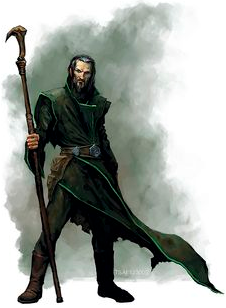
\includegraphics[width=0.40\textwidth]{evilSorcererAprentice}
	\newpage
	\section{Kampf um Ton}
	
	Als Sarasaus und Dalothor ihre rede beendeten und die Arbeiter sich auf die Wachen stürzten, bemerkten sie wie Prun und Taria in die Richtung eines Turmes sprinteten und beschlossen ihm zu folgen. Am Magier angekommen fing Prun an ihn mit Zaubern zu bombardieren. Der Magier zog ein rotes Amulett und fing einen Beschwörungszauber aufzusagen. Noch unten mit Wachen verwickelt bemerkte Lysanthir, dass auf dem Turm etwas passiert und Prun und Taria gegenüber jemand mit einem rot leuchtendem Amulett etwas vorhatte. In einem Versuch es zu unterbrechen schoss er ein Pfeil in Richtung des Magiers, dieser jedoch kam nicht mal ansatzweise an den Magier ran. 
	
	Kurz darauf beendete der Zauberer den Spruch und hielt sein Amulett an den Boden. Dieser fing an sich zu verflüssigen und es kamen 2 Ton Golem aus dem Boden. Der kleinere Golem sprang runter und fing an den isolierten Lysanthir anzugreifen. Doch nach ein paar Sprüngen über den Golem mit dem ein oder anderem Schwerthieb zerfiel der Golem wieder.
	
	Taria beschloss zunächst den großen Golem zu beschäftigen, damit Prun zeit hat, sich dem Magier zu widmen, da sie sich offensichtlich kennen, und eine offene Rechnung mit einander zu haben. Kurz darauf kamen auch Dalothor und Sarasaus an und kämpften mit Taria gegen den Golem. Prun schafft es eigenhändig den Magier zu erlegen. Als der Magier zu Boden fiel [wurde das Amulett recovered oder wurde es zerstört? - hebte er es auf oder sah wie das amulett zerstört wurde durch den fall], woraufhin er sich zum Golem wendete. Nach dem ersten Zauber schlug der Golem nach Prun, wodurch er großen schaden erlangte. Die anderen drei hackten auf dem Golem rum, bis Sarasaus mit einem Sprung den Golem in zwei teilte. 
	
	Die restlichen Wachen werden noch beseitigt und die Gruppe kommt wieder zusammen und finden Hilfin. Dieser ist höchst dankbar von den Tyrannen befreit zu werden und verrät ihnen, dass der Informant bei ihm das Pferd zurück gab und den sogenannten Zirkel suchte. Hilfin war sich nicht mehr ganz sicher, aber der Informant hatte etwas von einer neuen Waffe geredet, welche den Fürsten stürzen könne. Nach etwas überlegen fanden sie heraus, dass der Zirkel ihren Standpunkt in Langorion hat. Unmittelbar wollten sie sich auf den Weg dahin begeben.
	\newpage
	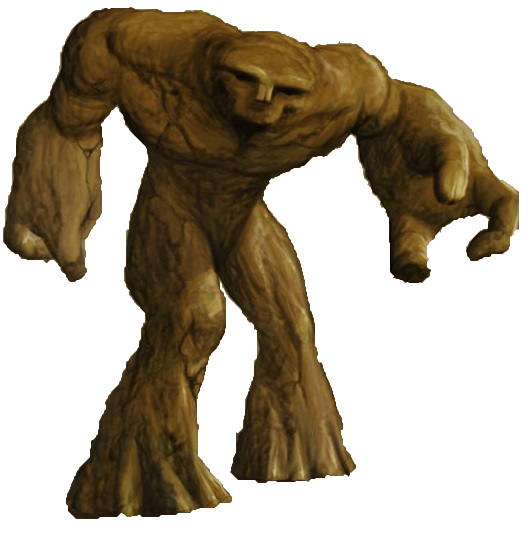
\includegraphics[width=0.40\textwidth]{unbakedGolemSmall}\par\vspace*{3cm}
	
	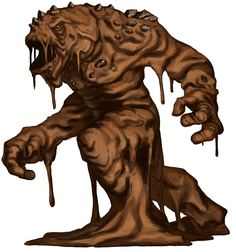
\includegraphics[width=0.40\textwidth]{unbakedGolemBig}\par
	\newpage
	
	
	
\end{document}